%Document vide aux normes de l'École nationale des Chartes
%Dernières modifications E. Rouquette (12/2023)


\part{Partie 3 : le code c'est la loi, régulations et limites à la découvrabilité}
%\setcounter{chapter}{0} % remet le compteur des chapitre à 1 

\chapter*{\enquote{Le code : c'est la loi}}

Le code, c’est la loi\index{Code is law} : « \textit{code is law} »\footcite[(nous avons consulté la version française disponible sur Framablog)]{lessig_code_2000}. Dans un article paru en 2000, Lawrence Lessig met le doigt sur un enjeu central du web : sa régulation\index{Régulation}. Or, le web, à la différence de nos sociétés, n’est pas régulé par des textes de loi et une constitution : non, ce qui régule le web c’est le code, c’est lui qui détermine s’il est facile ou pas d’accéder à un contenu, qui détermine si vous allez pouvoir découvrir cet incroyable vase grec, c’est lui encore qui décidera de votre orientation (l’exemple de \textit{Parcoursup} le montre). Si les règlements\index{Régulation} européens récents, tel que celui sur la protection des données tentent de réguler le web, force est de constater qu’ils sont limités et ne touchent qu’une infime fraction des interactions que nous avons avec ce dernier. Et comme le montre Laurence Lessig, parfois c’est bénéfique : c’est parce que le protocole \textit{TCP/IP} (qui permet l’échange de données) rend difficile d’associer une adresse IP (celle d’un ordinateur) à une personne que le web est un espace sans précédent de liberté d’expression ; mais c’est aussi pour cette raison que la haine en ligne est difficile à endiguer\footcite[§8 et § 9]{lessig_code_2000}.

Revenons aux origines du web pour comprendre pourquoi l’écosystème a été pensé, dès son origine, de façon si libertaire. Si internet a d’abord été, dans le contexte de la guerre froide, vu comme un moyen de relier de façon décentralisée différents ordinateurs afin d’améliorer la résilience des États-Unis en cas de guerre nucléaire\footcite{2024i}, le projet sera, finalement, surtout utilisé par les universités américaines (en témoigne la première carte du réseau visible ci-après), notamment pour optimiser l’utilisation des très couteux ordinateurs de l’époque.


\begin{figure}[h!]
	\centering
	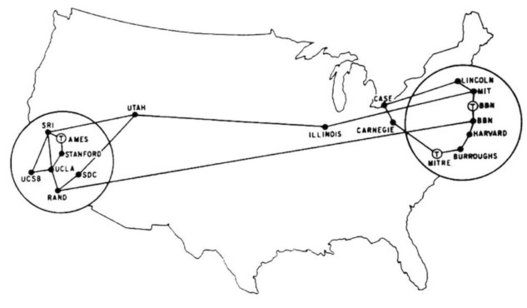
\includegraphics[width=0.8\textwidth]{images/image24.jpg}
	\caption{Carte d’ARPANET en 1972}
	\label{fig:image24}
\end{figure}

\begin{center}
	Depuis : \url{https://www.accessoweb.com/La-carte-de-Arpanet-en-1972-les-debuts-d-Internet_a8123.html}
\end{center}


Les mouvements libertaires, dont Stewart Brand\footnote{ Il est l’objet du livre de Fred Turner, « Aux sources de l’utopie numérique. De la contre-culture à la cyberculture, Stewart Brand un homme d’influence », trad. de l’anglais par Laurent Vannini, Caen, C\&F Éd., 2012, 432 p.}, l’un des pionniers d’internet faisait partie, s’intéressent à cette infrastructure, car ils se méfiaient des structures étatiques centrales et voyaient en internet un potentiel d’interactions libres sans interventions de ces dernières, car il était, dès sa conception, conçu sur un modèle décentralisé. Brand contribue à populariser l’idée que les ordinateurs personnels pouvaient contribuer à l’idéal libertaire en permettant à chacun de devenir autonome au sein d’un réseau mondial sans « tête »\footcite[§ 5]{goeta_fred_2013}.

Mais, pour revenir à l’article de Lessig, si internet et le web ont été pensés dès leurs débuts comme des espaces libres, cette approche n’est pas figée, « car le code n’est pas figé »\footcite[§ 6]{lessig_code_2000}, d’autres éléments peuvent être ajoutés pour permettre d’identifier à coup sûr l’auteur d’une publication par exemple. Comme le code détermine les valeurs d’internet, poursuit l’auteur, c’est en intervenant sur ce dernier qu’on peut les modifier ; il balaye les arguments, très actuels (le patron de X s’en est fait le parangon) selon lesquels on devrait choisir entre une régulation (par l’État par exemple) et son absence : or, le code régule, soit il protège la vie privée soit il promeut la surveillance, soit il laisse la haine en ligne être diffusée soit il tente de la limiter (X est un excellent exemple en la matière). L’auteur conclut son article, écrit en 2000 pour rappel, en expliquant que si l’État n’intervient pas, la régulation\index{Régulation} est placée du côté d’acteurs privés qui ont des objectifs bien différents\footcite[§ 28]{lessig_code_2000}. L’article illustre bien trois enjeux essentiels, que ce soit pour la découvrabilité et la diversité culturelle ou le web en général : le code c’est la loi\index{Code is law} donc il faut comprendre ses biais et problématiques afin de les contrer ; le code c’est la loi donc les institutions doivent s’en emparer, soit pour le réguler, soit pour utiliser son potentiel et ne pas passer à côté ; et enfin, le code c’est la loi donc les personnes qui l’écrivent doivent être conscientes des enjeux que sous-tendent leurs actions. L’objet de cette partie sera donc d’explorer, d’abord les éventuels biais et potentialités du web en matière de découvrabilité, ensuite les questions institutionnelles autour de ce dernier : de la formation des agents à la régulation\index{Régulation}, pour finir, nous nous intéresserons aux angles morts de la notion.

\chapter{Le web : prison ou fenêtre ouverte sur le monde ?}

\subsection{L'hyperchoix\index{Hyperchoix}}

Cette notion est centrale pour commencer cette partie sur le web. On peut la définir comme le fait de faire un choix parmi un grand nombre d’options. Dans son ouvrage « \textit{L’attaque des clones} »\footcite{durand2016}, Emmanuel Durand l’exemplifie avec \textit{Gangnam Style}, vidéo sortie en 2012 et qui en un mois a battu tous les records de visionnages sur \textit{YouTube}, devenant la première vidéo cumulant 1 milliard de vues qui, toujours selon l’auteur, vient révéler deux choses : l’incroyable possibilité de diffusion pour des artistes en dehors des circuits traditionnels et le caractère aléatoire de la notoriété « \textit{buzz} » qui en découle parfois. Pour lui, cette notion illustre le potentiel presque infini du web à se faire diffuseur d’œuvres qui ne l’auraient pas été autrement, dans le monde entier\footcite[§ 1 et § 4]{durand_chapitre_2016}. C’est une révolution : avant l’arrivée d’internet, l’accès aux œuvres de l’esprit était limité, même avec l’émergence, dans le courant des XIXe et XXe siècles des industries culturelles que sont la photographie, la presse ou encore le cinéma ; il était difficile pour des artistes d’acquérir une notoriété et d’être diffusé sans l’appui de grands éditeurs. Internet aurait donc accompli une véritable utopie : celle de l’accès pour tous et toutes (pas totalement, seuls environ 50 \% de la population mondiale ayant accès à internet)\footcite{2024h} à des œuvres et à des savoirs de façon quasi illimitée. Cela contribue, si l’on suit le rapport mondial de l’UNESCO intitulé « \textit{Repenser les politiques culturelles} »\footcite[cité dans Durand Emmanuel, \textit{l'attaque des clones}... § 10]{zotero-651}, à réduire les contraintes : à la fois sociales, géographiques et culturelles au sein des nations tout en ouvrant au niveau mondial le savoir et sa découverte.

Il est vrai que le web ainsi que l’essor de l’informatique personnelle permettent aux créateurs de publier de façon presque gratuite tout en leur donnant la possibilité de créer différemment. Par exemple, nous avons tous la possibilité de nous improviser monteur de vidéos, créateur de musique, illustrateur… Le tout de façon très simple et avec des couts très réduits. Cela a eu pour effet de remettre en cause (au moins en partie) le rôle des industries culturelles et notamment les diffuseurs qui décidaient avant de ce qui serait ou ne serait pas dans le monde culturel\footcite[§ 19]{durand_chapitre_2016}.

Mais cette facilité à publier et à mettre en ligne, et on l’a vu longuement déjà dans ce mémoire, peut aussi être un problème : celui de la masse, comment faire les bons choix ? Comment repérer les Mozart de demain ? Qui plus est quand les choix renvoient à volonté vers d’autres potentiels choix avec le système des hyperliens\footcite{noauthor_hyperchoix_nodate} et à une époque où près de la moitié du trafic mondial serait assuré par des robots et où ils sont en capacité de générer des contenus à volonté\footcite{ertzscheid2023} ?

Il faut donc poser la question de la sélection dans la prescription qui était auparavant la distinction au sein d’une production et qui devient un choix répondant aux attentes d’un consommateur au sein d’une offre pléthorique\footcite{ertzscheid2023}. Mais aussi celle de l’évaluation, qui n’est plus l’avis d’un expert qui désigne une valeur en recommandant ou non un contenu, mais une liste d’avis motivés par des critères, soit qualitatifs, « les plus aimés », soit quantitatifs, « les plus vus ». Car si l’écosystème numérique a permis de court-circuiter les systèmes de diffusion traditionnels, ces derniers n’ont pas totalement disparu et ont été remplacés par des groupes, en immense partie Américains, qui tentent de rassurer leur public avec des « discours d’ONG »\footcite[p. 3]{laugee__2013}, mais qui, quoiqu’on puisse en dire, ont besoin de trafic pour vivre, car ils reposent sur des modèles publicitaires et sur leurs capacités à être prescripteurs, on parle de « capitalisme linguistique »\footcite{kaplan_quand_2011}. C’est-à-dire, qu’au lieu de vendre un produit pour générer des profits, comme c’est le cas de manière classique, ces entreprises, et Google au premier chef, vendent des mots. Ces derniers ont aussi un cours en bourse, ainsi être placé en haut des résultats de recherche concernant le mot « football » sera plus cher pendant la coupe du monde qu’en plein été au moment où les compétitions font une pause (Google Maps fonctionne selon le même principe mais aussi Facebook)\footcite{kaplan_quand_2011}.

On a donc un hyperchoix\index{Hyperchoix} d’une part caractérisé par une quantité informationnelle immense, et de l’autre une « hyperindividualisation »\footcite[p. 3]{laugee__2013} qui vient la canaliser. Au final, la question qu’il convient de poser est celle de la réalité derrière la théorie : est-ce que le web a réduit ou augmenté la diffusion de la culture dans toute sa diversité ? C’est ce que nous tenterons d’observer dans notre prochaine partie en partant du concept de longue traine\index{Longue traine} (\textit{long tail}).

\subsection{Une longue traine ou une courte tête ?}

Le terme de longue traine\index{Longue traine} (\textit{long tail}) a été proposé en 2004 par Chris Anderson qui constatait alors que le web pouvait favoriser l’augmentation de la diffusion des contenus peu ou pas diffusés auparavant : de niche\footcite[§ 8]{benghozi_longue_2008}. Il convient de tenter, après 20 ans, de l’analyser et de l’objectiver, cela nous sera utile pour poursuivre notre réflexion sur l’écosystème qu’est le web et ses spécificités sur le plan de la découvrabilité. Ce que ce terme vient tenter d’exprimer, c’est la grande différence entre l’espace physique, limité, et l’espace numérique qui serait affranchi de toute contrainte spatiale. Pensons à l’exemple d’une librairie : dans un espace donné, elle sera capable d’afficher une vingtaine de milliers d’ouvrages, souvent dans la langue locale\footcite[§ 11 et § 12]{benghozi_longue_2008}. Ce concept repose sur deux effets : une offre qui s’élargit d’une part et de l’autre une recommandation\index{Recommandation} qui devient plus personnalisée, on l’a vu\footcite[§ 17]{bourreau2015a}.

Les chiffres semblent montrer que l’effet \textit{long tail} serait fantasmé et que ce qui serait plutôt mis en place est son exact contraire : l’effet \textit{short head}\index{Courte tête} : la majorité des consultations se feraient sur une partie infime des contenus. On avance souvent la proportion de 80/20 : 80 \% des contenus rassembleraient 20 \% des personnes et 20 \% des contenus 80 \% des personnes\footcite[§ 10]{bourreau2015a}. Il faut cependant nuancer ces chiffres, s’ils restent globalement vrais, il faut tout de même noter que 20 \% des contenus sur le web représentent une diversité bien plus importante que ce qui pouvait être le cas avant l’informatisation : la proportion est restée sensiblement la même, mais elle masque le fait que les chiffres du total de contenus différents consultés ont augmenté de façon très importante\footcite[§ 15]{bourreau2015a}. Dans tous les cas, il est très difficile de conclure à la réalité ou non de cet effet de longue traine\index{Longue traine}, les nombreuses études sur le sujet étant assez contradictoires et très dépendantes du secteur culturel concerné (on évoquera le cas spécifique du patrimoine culturel juste après)\footcite[tableau 1]{bourreau2015a}.

On peut néanmoins tenter, grâce à l’article de Marc Bourreau, Sisley Maillard, François Moreau « Une analyse économique du phénomène de la longue traine\index{Longue traine} dans les industries culturelles »\footnote{déjà cité plusieurs fois} d’expliquer les raisons de la limitation de l’effet \textit{long tail} observées. La première a été formulée par le sociologue MacPhee en 1963 : les gens moins familiers à un marché (par exemple la musique) qui représentent la majorité des consommateurs vont souvent diriger leur choix vers des valeurs plus sûres, déjà bien établies ; les experts, minoritaires, vont eux ventiler leurs choix entre, effectivement, des produits de niches, mais vont tout de même continuer à consommer des produits populaires. Donc in fine, les produits de niches seront plus rarement consultés\footcite[§ 29]{bourreau2015a}. La deuxième raison a déjà été évoquée longuement dans ce mémoire, il s’agit du concept d’économie de l’attention\index{Économie de l’attention}, quand un utilisateur a trop de choix, cela lui demande un coût cognitif élevé, il va donc préférer se tourner par mimétisme, là aussi, vers ce qui lui est soit recommandé : soit par un tiers (ou par son équivalent informatique que sont les classements « titres les plus vus » ou « titres les plus aimés » par exemple), soit par un algorithme (notre prochaine partie sera consacrée à évaluer leur rôle dans les prescriptions culturelles)\footcite[§ 39]{bourreau2015a}. Troisième raison, le manque d’information des consommateurs contribuerait, selon une étude d’Hendricks et Sorensen\footcite[§ 40]{bourreau2015a} (2009) à limiter la visibilité des contenus de niche. Ce qui serait le symptôme visible d’une limite qui reste importante, celle de l’exposition médiatique des titres qui reste réservée à une petite partie des producteurs de contenus culturels, notamment dans les médias traditionnels (limités par leurs grilles) qui conservent toujours un rôle de prescripteurs important\footcite[§ 41]{bourreau2015a}.

Pour revenir au domaine qui nous intéresse, le patrimoine culturel, si les études le concernant sont peu nombreuses et le climat bien moins concurrentiel que celui de la musique par exemple ; on peut néanmoins tirer quelques conclusions grâce à un article paru dans le \textit{Bulletin des bibliothèques de France} (\textit{BBF}) « La découvrabilité des collections numériques patrimoniales sous l’angle des usages de Gallica » (Bastard et Laborderie)\footcite{bastard2023}. Les auteurs y notent que 52 \% de la collection disponible en 2021 n’avait pas été consultée au cours de l’année, ce qui peut paraître important quoique bien plus faible que le ratio de 80/20 évoqué plus haut. Qui plus est, si l’on regarde dans le détail comme le font les auteurs en notant notamment que la presse, qui représente pourtant 76 \% de la collection numérisée, ne représente qu’un cinquième des consultations alors que 79 \% des livres numérisés ont été consultés au cours de l’année. La proportion documents consultés/documents disponibles atteint même 97 \% pour les vidéos et 91 \% pour les cartes\footcite[§ 8]{bastard2023}. Le phénomène de longue traine\index{Longue traine} est donc, semble-t-il, bien plus prégnant dans les usages numériques de Gallica que dans d’autres industries culturelles (les documents les plus consultés ont tout au plus 30 000 visites soit 1 \% du trafic !), et l’on peut tenter de l’expliquer par plusieurs raisons. La première est l’excellente repérabilité\index{Repérabilité} des collections de la bibliothèque nationale en ligne (déjà décrite) qui sont souvent recommandées par les moteurs de recherche (en témoigne l’image ci-après).


\begin{figure}[h!]
	\centering
	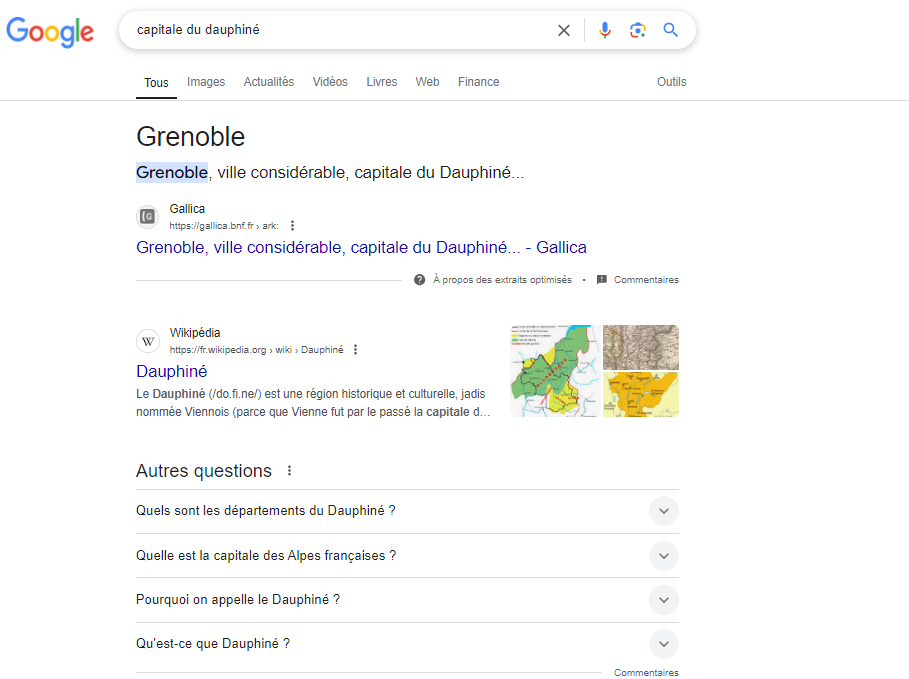
\includegraphics[width=0.8\textwidth]{images/image25.png}
	\label{fig:image25}
\end{figure}



La deuxième raison que l’on peut noter est l’impossibilité pour les utilisateurs de voir les \enquote{documents les plus consultés}, les documents mis en avant sur Gallica le sont par l’équipe éditoriale du site, jamais par rapport à leur audience (impossibilité de l’effet de mimétisme décrit plus haut). Poursuivons avec le fait que Gallica est consultée en majorité par des experts ; de fait, selon une enquête de 2020 menée par l’Observatoire des publics de la Bibliothèque\footnote{ Comme l’écrivent les auteurs, ces résultats ne sont pas forcément le reflet des publics réels de Gallica, mais plutôt de ceux désireux d’améliorer le service et qui le connaissent donc assez bien.} un tiers des usagers du site seraient des chercheurs, un autre tiers serait composé d’amateurs passionnés de science et de savoir (généalogistes, historiens amateurs, etc.) et un autre tiers se répartirait entre professionnels des bibliothèques et visiteurs ayant fréquenté l’établissement, or, comme le montrent les travaux de MacPhee cités plus haut, les experts sont les plus enclins à consulter des contenus « de niche ». Enfin, comme l’exposition médiatique des contenus numérisés dans Gallica est quasi nulle, cela ne contribue pas à en faire émerger certains au profit d’autres. On pourrait se risquer à écrire que la différence fondamentale entre Gallica et les autres industries culturelles qui fait que l’effet longue traine\index{Longue traine} s’observe de façon assez clivante est que le site n’est pas construit selon des logiques marchandes : l’objectif de la bibliothèque nationale n’est ni de vendre de l’espace publicitaire ni de faire rester les internautes sur son site, elle n’a donc aucun intérêt à favoriser un contenu plutôt qu’un autre. En effet, comme évoqué dans l’introduction, si le code est la loi, il s’agit bien de choix de la part des institutions ou des entreprises que de l’orienter vers telle ou telle direction. Nous verrons dans la partie suivante consacrée à la notion de bulle de filtres (et donc à la recommandation\index{Recommandation} algorithmique) que cela s’applique aussi tout à fait.

\subsection{Lutter contre la \enquote{bulle de filtre\index{Bulle de filtre}}}


Depuis quelques années, le phénomène théorisé en 2011 par Eli Pariser de \enquote{Bulle de Filtre}\index{Bulle de filtre} fait énormément parler de lui, il se définit comme un enfermement algorithmique des personnes par le biais d’une personnalisation trop importante. Il nous semble important de revenir en détail sur ce concept, car la découvrabilité est souvent évoquée comme une réponse aux problèmes qu’il pose et qui sont de deux ordres : premièrement un auto-renforcement des opinions politiques et clivages sociétaux, on parle souvent de radicalisation ; et deuxièmement, une perte de diversité culturelle.

Commençons par évoquer le premier cas, qui est bien décrit par Antoinette Rouvroy et Thomas Berns en 2013 dans leur article sur la \textit{gouvernementabilité algorithmique} qu’ils définissent comme un double mouvement composé de la création d’un \enquote{double statistique} du monde \enquote{qui redessine les hiérarchies classiques} et \enquote{l’évitement de toute confrontation avec les individus dont les occasions de subjectivation se trouvent raréfiées}\footcite{rouvroy_gouvernementalite_2013}. Ce phénomène s’est illustré lors du retentissant scandale dit \enquote{Cambridge Analytics} qui, en 2018 a éclaté au grand jour, révélant que les données d’entre 30 et 70 millions d’utilisateurs de Facebook ont été utilisées à leur insu afin d’influer sur leur vote à la présidentielle en ciblant la publicité électorale ou en modifiant les déplacements des candidats républicains\footcite{noauthor_ce_2018}.

Dans leur article de 2023, \enquote{De l’information aux industries culturelles, l’hypothèse chahutée de la bulle de filtre}\index{Bulle de filtre}\footcite{farchy_linformation_2023}, Joëlle Farchy et Steven Tallec reviennent sur ce concept afin de tenter de voir si l’hypothèse formulée en 2011 par Eli Pariser \enquote{souvent sur base d’anecdotes}\footcite[§ 5]{farchy_linformation_2023} est vérifiable par des travaux computationnels et empiriques. Il nous semble utile ici de résumer leurs conclusions, car avoir une compréhension fine de la notion de bulle de filtre\index{Bulle de filtre} est essentiel pour bien comprendre ce que peut, ou pas, la découvrabilité pour la contrer. Ils commencent par évoquer une étude de Robert Epstein et Ronald Robertson\citein[§ 15]{epstein2015}{farchy_linformation_2023} qui a prouvé que si l’on soumet un groupe d’individus à un moteur de recherche dont les résultats sont orientés vers un candidat en particulier, celui-ci sera plus enclin à voter pour ce dernier ; puis poursuivent avec une étude sur les réseaux sociaux\citein[§ 16]{bakshy2015}{farchy_linformation_2023} qui montre que, non seulement la principale source d’information des personnes étudiées sont les réseaux sociaux, mais qu’en plus ces derniers sont effectivement vecteurs de contenus avec lesquels l’utilisateur est en accord. C’est évidemment relié au concept d’économie de l’attention\index{Économie de l’attention} et au modèle économique des plateformes : puisque leur objectif est de faire rester le plus longtemps possible les utilisateurs, leur montrer des contenus avec lesquels ils sont en accord est profitable, par ailleurs, cela permet d’alimenter de façon plus fine la publicité ciblée\footcite{noauthor_bulles_nodate}. Les mêmes résultats sont observés sur \textit{YouTube} qui est décrit par Zeynep Tufekci comme un \enquote{grand radicalisateur}\citein[§ 18]{tufekci2018}{farchy_linformation_2023} qui amplifierait la visibilité de vidéos sensationnalistes et complotistes pour capter l’attention de son public.

S’il est clair, pour les auteurs, qu’on ne peut nier le phénomène, ces derniers nuancent cependant son impact réel, car les études ne portent à chaque fois que sur un canal de communication et non sur l’environnement médiatique global des personnes, qui ont — de toute manière — tendance à s’enfermer d’eux-mêmes dans des bulles de filtres, car ils écartent les opinions qu’ils ne souhaitent pas voir\citein[§ 26]{garrett2009}{farchy_linformation_2023}: de même qu’un lecteur de \textit{L’Humanité} n’aurait jamais l’idée d’acheter le \textit{Figaro}, il n’aura pas non plus envie de voir des articles qui vont à l’encontre de ses valeurs en ligne. Ils évoquent aussi l’article de 2015 qui, en s’appuyant sur un échantillon de 10 millions d’utilisateurs de Facebook, a démontré que ce sont les comportements individuels qui influencent le plus les opinions politiques, notons toutefois que cet article a été écrit par des chercheurs de… Facebook ! Les auteurs notent aussi \enquote{des internautes enfermés minoritaires} : 1 \% des utilisateurs de Twitter ont ainsi consulté 80 \% des fausses informations selon une étude de 2019\citein[§ 27]{grossetti2019}{farchy_linformation_2023}; comme elles sont générées par la sphère complotiste, le phénomène de bulle de filtre\index{Bulle de filtre} fait que — justement — elles y restent.

En fin de compte, l’article confirme l’existence de bulles de filtres, mais en proposant une analyse méthodique, il remet aussi en question les craintes exprimées de radicalisation de la société. Il est en revanche intéressant de noter que la suite de l’article s’intéresse à la question de la diversité culturelle. Le principe est similaire : puisque l’objectif des plateformes (et sites marchands vendant des contenus culturels) est de conserver leur public, vont-elles donner à voir uniquement les choses dont elles sont sûres que leur public appréciera, et donc plutôt des choses très connues et peu diverses ? Par ailleurs, vont-elles mettre en avant certains contenus qu’elles produisent elles-mêmes (Netflix est aussi producteur par exemple) ?

Là encore, l’article nuance en prenant deux exemples : Spotify et Netflix, le premier au catalogue\index{Catalogue} immense (80 millions de titres) et l’autre au catalogue\index{Catalogue} plus réduit (5 272 titres) ; pour le premier, des études ont clairement démontré que les radios générées à la demande de l’utilisateur ne favorisaient en rien la découverte ; en revanche les playlists \enquote{découvertes de la semaine} jouent bien leur rôle (elles auraient permis, en quelques mois, à quarante millions de personnes de consulter 5 milliards de morceaux nouveaux)\footcite[§ 2]{durand_chapitre_2016-1}. Pour ce qui est du second, il faut noter que la page d’accueil ne propose qu’une petite fraction du catalogue\index{Catalogue} (entre 11 et 20 \%)\citein[§ 47]{Chaire Pluralisme culturel et éthique du numérique (PcEn), mai 2022}{farchy_linformation_2023} et qu’une part encore plus faible est réellement consultée. En revanche, les utilisateurs sont ciblés de façon extrêmement fine et catégorisés dans des \enquote{communautés}, allant jusqu’à changer les vignettes illustrant les contenus en fonction des profils\footcite{noauthor_algorithmes_nodate}. Il y a donc bien un effet bulle de filtre\index{Bulle de filtre} sur Netflix et Spotify, mais il faut le relativiser : sur Spotify, les playlists créées par les équipes éditoriales (aidées par des algorithmes) permettent aux utilisateurs de consulter une assez grande part du catalogue\index{Catalogue} et de \enquote{sortir de leur zone de confort}, tout en restant il est vrai sur des titres majoritairement connus. Du côté de Netflix, s’il est vrai que les communautés voient des contenus très spécifiques, leur nombre très important (entre 1300 et 2000)\citein[§ 48]{rodriguez2017}{farchy_linformation_2023} fait que le catalogue\index{Catalogue} de la plateforme est visionné en grande partie : en revanche, chacun est enfermé dans \enquote{sa communauté}\footnote{Voir à ce propos le, déjà cité, témoignage d'April Joyner : \url{https://www.marieclaire.com/culture/a18817/netflix-algorithms-black-movies/ }}.

Il semble que pour le cas du patrimoine, la conclusion soit ici la même que précédemment, comme les institutions dans le domaine n’ont \enquote{rien à vendre}, elles n’ont pas d’intérêt à faire en sorte que d’hypothétiques algorithmes de recommandation\index{Recommandation} (car il faut reconnaître que les exemples manquent en ce domaine) favorisent un contenu plutôt qu’un autre. Fort est à parier que si ces dernières mettent en place de tels dispositifs, qui sont à l’origine plutôt un moyen d’objectiver la recommandation\index{Recommandation} plutôt que de créer l’enfermement algorithmique (relatif) décrit, ils seraient plutôt des facilitateurs de rebonds entre différents éléments des collections, car il est vrai que ce taux paraît assez faible (entre 1 et 3 par session de navigation) sur Gallica\footcite{bastard2023} plutôt que des facteurs d’enfermement. Mais alors pourquoi ne sont-ils pas plus massivement déployés dans les institutions qui auraient pourtant beaucoup, leurs usagers surtout, à gagner à cela ? Il semble qu’il faille aller poser la question de ce que peuvent les institutions en la matière, que ce soit pour réguler l’écosystème que nous venons de décrire, ou encore pour mieux le mettre à profit.

\chapter{Difficultés institutionnelles}

\subsection{Une nécessaire acculturation au numérique et des tabous à lever}

La découvrabilité des contenus culturels à l’ère numérique se heurte à plusieurs limitations institutionnelles, dont les manques d’acculturation\index{Littératie numérique} numérique et la présence de certains tabous au sein du secteur culturel. Le rapport de la Mission franco-québécoise sur la découvrabilité de 2020 en fait d’ailleurs l’un des leviers majeurs à activer pour les pouvoirs publics afin d’améliorer la découvrabilité des contenus culturels francophones. 

Ce dernier note tout d’abord un fort besoin de mise en commun des expertises et bonnes pratiques dans tout le domaine culturel, par exemple, les professionnels du patrimoine, spécialisés dans l’indexation et les métadonnées pourraient apporter une expertise essentielle en matière de repérabilité\index{Repérabilité} (on l’a vu) et les professionnels de l’audiovisuel apporter la leur en matière de recommandation\index{Recommandation}, ce qui aurait pour effet d’améliorer la découvrabilité dans les deux sens.\footcite[p. 31]{ministeresdelaculturefranceetquebec2020} On peut aussi imaginer de casser les silos informationnels, non seulement sectoriels comme on l’a vu en parlant de portails et de politiques \textit{data-driven} (cf. partie 2), mais aussi de façon plus large dans tout l’écosystème culturel en créant des synergies. C’est ce que met en place le Pass Culture, dispositif créé en 2019 qui propose aux jeunes de 15 et 18 ans un crédit de 500 € qu’ils peuvent dépenser dans le secteur culturel de leur choix (films, livres, patrimoine, musique…). Le dispositif est accompagné d’une application qui a pour objectif principal de faire découvrir à son public des contenus les plus divers possibles. Outre le fait qu’elle soit dotée d’un algorithme de recommandation\index{Recommandation} et qu’une équipe éditoriale vienne aussi assurer ce rôle, il faut noter la présence très intéressante d’un \enquote{score de diversification}, visible par les utilisateurs, qui augmente avec le nombre de catégories différentes visitées.\footcite{martinstocker} On a donc, grâce à ce dispositif dit de \enquote{ludification}\footcite{2024g}, une augmentation de la diversité (observée depuis le début du dispositif) des contenus culturels consommés par les utilisateurs qui ne se soucie pas des frontières classiques évoquées plus haut, jouant ainsi le rôle de portail\index{Portail} d’accès aux contenus culturels, quel que soit le domaine.

Le rapport revient aussi sur l’importance centrale de la formation à cette notion, encore très mal connue (surtout du côté français) et aux enjeux qui la sous-tendent (pour rappel : disponibilité\index{Disponibilité}, repérabilité\index{Repérabilité} et recommandation\index{Recommandation}) en créant une véritable culture de la donnée dans les institutions.\footcite[p. 23]{ministeresdelaculturefranceetquebec2020} Donc des compétences en matière de compréhension des technologies de l’information et de la communication (algorithmes au premier chef), des méthodes de marketing numérique (référencement\index{Référencement}) et des sciences de l’information que sont l’indexation et la gestion des métadonnées (dans ce domaine, les institutions patrimoniales ont une avance certaine). Ces dernières sont réparties en 4 piliers visibles dans l’image ci-après, extraite du rapport sur la découvrabilité et recréée par nos soins.\footcite[p. 21]{ministeresdelaculturefranceetquebec2020}



\begin{figure}[h!]
	\centering
	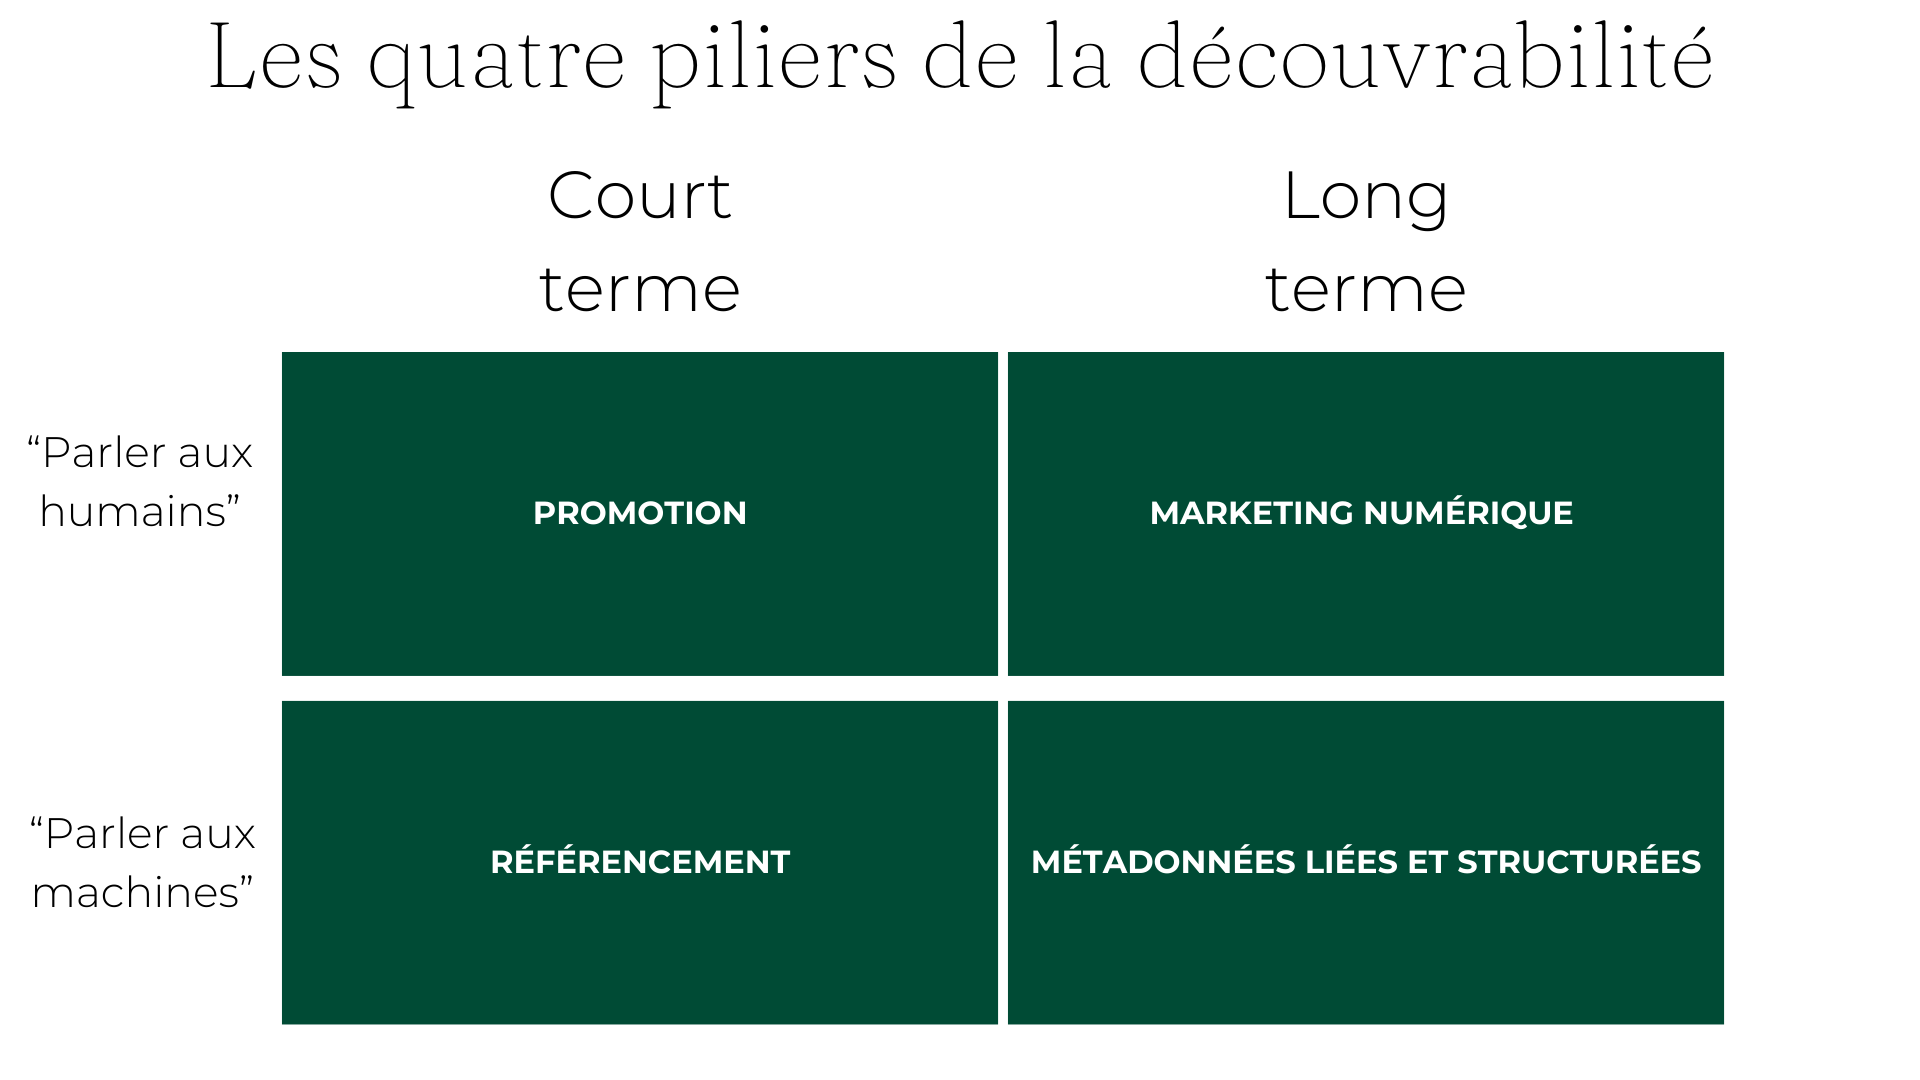
\includegraphics[width=0.8\textwidth]{images/image26.png}
	\caption{Les quatre piliers de la découvrabiltié}
	\label{fig:image26}
\end{figure}



Il y a donc un manque de formation des professionnels de la culture aux enjeux de découvrabilité qui est parfois compensée par ces derniers qui ont à leur disposition en ligne des formations gratuites souvent proposées par les GAFAMS\footnote{Google Apple Facebook Amazon Microsoft }, ce qui pose non seulement la question de la dépendance à ces outils, mais aussi celle de la pertinence de telles formations, pas toujours adaptées aux cas d’usages spécifiques des secteurs culturels.\footcite[p. 22]{ministeresdelaculturefranceetquebec2020} Évidemment, cette question de la formation est avant tout celle des moyens mis à disposition des institutions pour accomplir leurs missions, car il faut des professionnels qualifiés pour les remplir et donc de l’argent pour les recruter. Par ailleurs, la stratégie de promotion des contenus culturels passe parfois par l’achat d’espaces publicitaires en ligne ou la mise en place de partenariats, par exemple avec des influenceurs dont le rapport note l’importance croissante.\footcite[p. 22]{ministeresdelaculturefranceetquebec2020} 

Il faut aussi noter un frein simplement mentionné dans le rapport : celui de pratiques professionnelles qui \enquote{méritent d’être reconnues}.\footcite[p. 21]{ministeresdelaculturefranceetquebec2020} De fait, ces dernières et plus généralement le domaine du numérique, à cause de la complexité d’appréhension de leurs effets, parfois obscurs (d’où l’importance de l’explicabilité du code et de ses effets qui sera l’objet de la partie juste après) surtout dans le cas de la recommandation\index{Recommandation}, sont souvent assez mal vues et mal perçues par les institutions patrimoniales et leurs usagers. En témoigne le fait que la seule institution patrimoniale lauréate de l’appel à projets pour la découvrabilité en ligne des contenus culturels proposé par le ministère de la Culture soit le projet, déjà cité, data.bnf.fr\footcite{noauthor_decouvrabilite_2024}; et même s’il est vrai que l’institution est une tête de réseau qui fédère bon nombre d’acteurs au travers notamment du catalogue\index{Catalogue} collectif de France ou de Gallica (tous deux moissonnés par data.bnf.fr). D’autres acteurs du secteur patrimonial pourraient bénéficier de ces moyens pour améliorer la découvrabilité de leurs contenus culturels et notamment les musées.  

Il faut toutefois prendre en compte, qu’il est difficile voire impossible pour les institutions culturelles de rivaliser avec les moyens des GAFAMS en matière de découvrabilité de leurs contenus (par exemple Netflix investit 3 milliards par an rien qu’en marketing digital)\footcite[p. 23]{ministeresdelaculturefranceetquebec2020}, cependant, ces dernières ont des atouts qu’il ne faut pas négliger en la matière : la confiance des utilisateurs à leur égard bien sûr, mais aussi la possibilité de voir des régulations mises en place pour les favoriser, elles seront l’objet de notre prochaine partie.


\subsection{Règlementer pour favoriser la découvrabilité}

La question des régulations dans le domaine de la découvrabilité des contenus culturels est complexe et souvent négligée. Bien qu’ils ne constituent pas une solution universelle, certains ajustements règlementaires pourraient effectivement améliorer la visibilité des contenus culturels en ligne. Certains secteurs tels que la \textit{musique} et le \textit{cinéma} ont rapidement vu des règlementations sous forme de quotas être mises en place, tel est le cas par exemple de la loi Toubon qui a été votée en 1994 et qui impose aux radios de réserver une part variable (entre 40 et 10 \%) à la chanson française et aux artistes émergents\footcite{noauthor_comprendre_2016}. Plus récemment, le législateur européen s’est emparé de la question (directive services de \textit{médias audiovisuels}, traduite en 2021 en droit français) en demandant aux \textit{médias à la demande} de promouvoir les œuvres européennes en \enquote{facilitant l’accès à celles-ci} notamment, propose le texte, en les mettant sur la page d’accueil et en permettant aux utilisateurs de filtrer les œuvres européennes\footcite{noauthor_directive_2019}. Ce texte s’attaque donc directement à l’enjeu de découvrabilité en imposant, en plus des quotas, de réserver une place facilement repérable aux contenus européens. Ce type de réglementation de marché, assez classique, doit être complété, selon Mira Bruni (dans un rapport sur la diversités des contenus à l'ère numérique) d'une réglementation par les algorithmes, c'est-à-dire \enquote{des interventions ciblées avec des outils qui favoriseraient l'exposition à la diversité des contenus en augmentant la visibilité et la découvrabilité de certains types de contenus au moyen de processus éditoriaux effectués par les algorithmes.}\footcite{canadien2019}. Son propos est complété par M. Napoli qui indique qu'il est important de réglementer \enquote{l'intégration verticale}\footnote{L'intégration verticale est un concept dans lequel une entreprise contrôle plusieurs partie du processus économique, par exemple, dans notre cas : Netflix est à la fois producteur de contenus mais aussi diffuseur par le biais de sa plateforme, favorisant ainsi, algorithmiquement, les contenus produits  en propre. - Wikipédia, intégration verticale, consulté le 25/08/2024} dans le secteur culturel, car cette dernière favoriserait trop les contenus produits en propre par les plateformes. Par ailleurs, selon les auteurs du rapport cité plus haut, \enquote{l'autorégulation des plateformes en ligne a révélé ses limites}, il faut donc que les gouvernements aillent plus loin que l'incitation à la régulation\index{Régulation} et viennent directement réguler les plateformes, espaces privés dans la sphère publique qu'est le web ayant leurs propres règles.\footcite{canadien2019}.  

Si les secteurs cités plus hauts, parfois qualifiés de privilégiés, bénéficient d’un encadrement législatif fort qui tend à préserver la diversité culturelle (même si elle n’est que relative puisqu’elle veut surtout soutenir les productions nationales) ; ce n’est pas le cas pour tous. C’est assez logique dans le cas patrimonial où l’objectif est plutôt, on l’a déjà largement décrit, de briser les frontières entre les collections pour permettre leur diffusion à une large échelle, mais il faut tout de même noter que — et c’est plus une question de moyens financiers que de régulations — des institutions de petite taille voient le patrimoine qu’elles conservent invisibilisé par les \enquote{\textit{superstar}} que sont les grandes institutions, souvent parisiennes pour le cas de la France. La réglementation qui pourrait favoriser la visibilité et la découvrabilité des contenus de toutes les institutions serait plutôt sous forme de programmes d'aide à la numérisation, comme le plan de numérisation qui était au départ sous forme d'appels à projets annuels proposés par l'administration centralisée et qui a été déconcentré en 2018 dans les Directions régionales des affaires culturelles (DRAC) afin de cibler les institutions en région, plus en retard dans les chantiers de numérisation que les institutions centrales.\footcite{zotero-686} On peut aussi noter le Plan d'action pour le patrimoine écrit (PAPE) coordonné par la BnF et les pôles régionaux de coopération des acteurs du livre et de la lecture et région (par exemple Mobilis pour la région Pays-de-la-Loire)qui vise au signalement \enquote{des collections patrimoniales : manuscrits et archives sans limitation de date, livres imprimés jusqu’en 1830 pour l’ensemble des bibliothèques territoriales, livres imprimés jusqu’en 1914 pour les bibliothèques territoriales classées ou relevant d’une collectivité de plus de 500 000 habitants, fonds locaux et spécialisés, sans limitation de date.}\footcite{zotero-688}. Tous les ouvrages signalés ainsi sont intégrés au catalogue\index{Catalogue} collectif de France (CCFr), hébergé par la BnF, qui rassemble ainsi en un point d'entrée unique des collections éparpillées sur tout le territoire, permettant à des bibliothèques de taille très modeste d'avoir une visibilité à l'échelle nationale. 

\subsection{La question des droits d'auteurs}

Concentrons-nous dans cette partie sur une règlementation absolument centrale en ce qui concerne la découvrabilité des contenus patrimoniaux : le droit d’auteur\index{Droit d’auteur}. Car comme le rappelle très bien le rapport sur la découvrabilité déjà cité, \enquote{Vecteur indispensable de découvrabilité en ligne, les images sont, pour certains secteurs (\textit{arts visuels} et \textit{patrimoine}), souvent protégés par des droits d’auteur qui en empêchent l’exploitation en ligne, à moins de disposer de budgets considérables pour lever ces droits, ou d’une meilleure répartition de la valeur issue de l’exploitation de ces images par les plateformes. C’est un enjeu devenu encore plus névralgique depuis que Google propose toujours plus d’images dans les résultats de recherche pour tenir compte de cette préférence des utilisateurs}\footcite[p. 32]{ministeresdelaculturefranceetquebec2020}.

Rappelons donc ici le cadre légal actuel brièvement (il concerne toute l’Union européenne, on parle de droit continental). Le droit d’auteur\index{Droit d’auteur} est divisé en deux parts : les droits moraux d’abord, qui sont perpétuels, inaliénables et imprescriptibles et qui incluent le droit de paternité (l’auteur d’une œuvre sera toujours reconnu comme tel) et le droit au respect de l’œuvre (qui la protège contre toute modification susceptible de la dénaturer) ; les droits patrimoniaux quant à eux permettent à l’auteur de tirer des revenus de son œuvre, ils incluent le droit de reproduction (copie de l’œuvre) et de représentation (visibilité publique de l’œuvre), en France ils durent 70 ans sauf à de rares exceptions (notamment pour les auteurs morts pour la France)\footcite{zotero-323}. Cet arsenal législatif est complété par la directive européenne sur le droit d’auteur\index{Droit d’auteur} et les droits voisins dans le \textit{marché unique numérique} (adoptée en 2019 et transposée en droit français en 2021), qui renforce ces protections. Cette directive introduit des mécanismes pour que les créateurs soient équitablement rémunérés pour l’exploitation de leurs œuvres en ligne, en particulier lorsqu’elles sont utilisées par des plateformes comme \textit{YouTube} ou \textit{Google}\footcite{noauthor_directive_2019}. 

Maintenant que le cadre est posé, il faut noter quelques éléments importants. Premièrement, le droit d’auteur\index{Droit d’auteur} actuel constitue une limitation assez importante dans la disponibilité\index{Disponibilité} des collections culturelles en ligne, et notamment pour les musées d’art contemporain à l’image du \textit{Centre Pompidou} qui a numérisé et mis en ligne une grande partie de sa collection et a pour cela dû faire un nombre très important de demandes d’autorisations, car la majeure partie des œuvres étaient encore protégées par le droit d’auteur\index{Droit d’auteur}\footcite[§ 10]{bermes_parcours_2013}. Si le musée a pu \enquote{se permettre} humainement de faire toutes ces demandes, ce n’est pas le cas de toutes les institutions qui n’ont parfois que peu de personnel à leur disposition et qui doivent déjà faire face à des coûts de numérisation parfois (très) élevés. Pourquoi ne pas alors étendre la directive européenne citée plus haut pour que les plateformes visées paient une contribution, finalement assez logique, aux institutions patrimoniales dont elles diffusent les données afin que cela contribue aux frais de numérisation et de maintenance ? C’est d’ailleurs ce que fait Google avec \textit{Wikipédia} en finançant l’association en échange d’un accès plus facile et perfectionné à la base de données \enquote{\textit{Wikidata}}\footcite{noauthor_google_nodate}. 

Pour finir sur la question des règlementations, il faut aussi noter que les institutions ont souvent tendance à elles-mêmes s’en imposer et sont assez frileuses contrairement aux grands groupes. À l’image de Google qui, à travers son projet \textit{Google Books}, a tenté de contourner les lois sur le droit d’auteur\index{Droit d’auteur}, notamment en ce qui concerne les œuvres orphelines qui sont des œuvres pour lesquelles le ou les détenteurs des droits d’auteur ne peuvent pas être identifiés ou retrouvés, rendant ainsi toute exploitation légale complexe. Google, en numérisant massivement des livres sans avoir toujours obtenu l’accord des titulaires des droits et en supposant, par défaut, que les ayants droit étaient d’accord pour voir leurs œuvres diffusées, charge pour eux d’indiquer le contraire (on parle d’OPT-OUT). Cependant, cette approche a rapidement rencontré une opposition farouche, notamment de la part des auteurs et des éditeurs qui voyaient dans cette démarche une atteinte directe à leurs droits. La justice américaine a fini par trancher en 2011, estimant que Google ne pouvait pas se permettre de publier ces œuvres sans un accord préalable\footcite{ertzscheid2019}. Quel que soit le résultat, cet exemple illustre bien comment une entreprise de la taille de Google a tenté de \enquote{jouer} avec les lois existantes, dans l’espoir de créer un précédent favorable pour ses intérêts. Pour sortir d’une posture manichéenne où Google serait le \enquote{méchant}, il faut tout de même noter que si l’entreprise avait gagné ce procès cela aurait été une formidable opportunité de diffusion d’œuvres qui jusque-là étaient totalement introuvables en plus, évidemment, de générer des revenus très importants à l’entreprise américaine. Un autre exemple montre bien qu’il faut nuancer cela, c’est celui d’un autre procès opposant \textit{Internet Archive} (fondation archivant le \textit{web}) et quatre grands éditeurs internationaux (\textit{Hachette}, \textit{HarperCollins}, \textit{John Wiley \& Sons} et \textit{Penguin Random House}) qui a débuté en 2020, les éditeurs accusant la fondation de diffuser des livres sans respecter le droit d’auteur\index{Droit d’auteur}. Car la fondation effectue des sauvegardes de la quasi-totalité des sites \textit{internet} depuis sa création, mais aussi des copies de livres et en 2020, elle avait mis en place un service de prêt gratuit (pendant la pandémie et la fermeture des bibliothèques) sans limites d’utilisateurs simultanés pouvant emprunter les ouvrages. Pour les éditeurs : il s’agit purement et simplement d’un piratage de masse là où la fondation argue du fait qu’elle respecte le droit d’auteur\index{Droit d’auteur} en restant dans un \enquote{\textit{fair use}} (usage raisonnable, notion de droit américain qui prévoit des exceptions au droit d’auteur\index{Droit d’auteur} pour faciliter la diffusion des idées)\footcite{noauthor_aux_2023}. Au final, \textit{Internet Archive} a perdu ce procès et a donc dû retirer ces livres de sa bibliothèque\footcite{noauthor_condamnee_nodate}.

Si ces deux exemples peuvent tout à fait justifier la peur qu’ont les institutions de \enquote{jouer} avec les règlementations, on peut tout de même parfois se désoler de leur pusillanimité en la matière, et même si, par définition, il est difficile de trouver des exemples de projets avortés par des institutions du fait de leur frilosité, on peut tout de même prendre un exemple vécu pendant notre stage. Nous avions noté que la carte interactive des contenus présentée en partie 2 était un excellent moyen de valoriser les collections de la RTS en ligne, car souvent la première recherche que l’on effectue est simplement le nom de notre commune de naissance, mais on nous a beaucoup dit — et à raison sûrement — qu’il n’était pas envisageable de la rendre accessible au public, car cela pourrait poser des problèmes pour l’institution, car cela risquait de rendre visible le fait que la majorité des sujets diffusés par la RTS concernaient les cantons de Genève et de Vaud, ce qui est assez logique compte tenu de la population de ces deux cantons (qui plus est, le canton du Jura n’est indépendant que depuis 1978 et n’existait pas avant cette date), mais par peur d’une réaction négative des auditeurs, dans un contexte assez tendu pour la RTS (qui devra faire face à une votation qui vise à réduire la redevance à 200 francs en 2025). Il est vrai que donner une vision d’ensemble des collections n’est donc pas forcément une bonne chose politiquement, car cela renseigne sur les pratiques de conservation. Mais tout de même, si l’on avait pris le temps de l’explication et de la justification, le public aurait sûrement très bien compris cette sur-représentation de certains territoires et l’outil aurait pu être très utile. Notons aussi, sans disposer d’informations précises sur le sujet, que le projet \textit{data.ina.fr} qui vise à proposer des statistiques sur les contenus conservés par l’institution qui devait être lancée en juin de cette année\footnote{C'est en tout cas ce qui a été annoncé lors d'une visite à l'INA en janvier dernier} ne l’est toujours pas : peut-être pour des raisons similaires à celles évoquées pour la RTS ? L’explication du fonctionnement des algorithmes et outils, surtout avec l’émergence des outils d’intelligence artificielle\index{Intelligence artificielle}, revêt donc une importance capitale. Mais est-ce que la notion de découvrabilité peut aussi s’appliquer à découvrir de façon pertinente le fonctionnement des algorithmes et du code en général ? Ce sera l’objet de notre prochaine partie.


\chapter{Les angles morts de la notion de découvrabilité}

\subsection{Découvrabilité appliquée au code : l'explicabilité}

Dans sa revue des cinq grands enjeux de l’intelligence artificielle\index{Intelligence artificielle}, le journal \enquote{Polytechnique insight} note l’importance de \enquote{justifier les décisions prises par un algorithme}\footcite{noauthor_nouveaux_nodate}, ce qu’on peut tout à fait rapprocher de la notion d’explicabilité du code qui se définit comme suit : \enquote{capacité de mettre en relation et de rendre compréhensible les éléments pris en compte par le système pour la production d’un résultat.}\footcite{zotero-315}. Cette notion prend une importance croissante avec le développement de l’intelligence artificielle\index{Intelligence artificielle}, en témoigne le rapport Villani (2018) français et son intégration à la stratégie européenne en matière d’intelligence artificielle\index{Intelligence artificielle}\footcite[p. 14]{maxwell_comment_2020}. La notion est d’ailleurs existante dans le droit français, les algorithmes de service public déjà évoqués sont en effet, au même titre que les agents, redevables de leurs actions. \enquote{Les administrations qui conçoivent et utilisent des algorithmes publics doivent donc “rendre des comptes” de leur utilisation auprès des individus concernés, mais aussi de la société dans son ensemble.}\footcite{noauthor_algorithmes_nodate-1}. 

Le rapport \enquote{Flexible and Context-Specific AI Explainability: A Multidisciplinary Approach} écrit par Valérie Beaudouin, Isabelle Bloch \textit{et al.}\citein[p. 14]{beaudouin2020}{maxwell_comment_2020} distingue quatre facteurs d’explicabilité : le destinataire (utilisateur, régulateur, expert…) ; le niveau d’importance de l’algorithme (besoins différents entre expliquer les raisons d’un crash de voiture autonome et les résultats de Google) ; le cadre légal et l’environnement de déploiement (application critique, besoin d’un usage facilité au maximum, etc.). Isabelle Bloch, titulaire de la chaire en intelligence artificielle\index{Intelligence artificielle} de Sorbonne université, note (propos recueillis par Sophy Caulier)\footcite{noauthor_nouveaux_nodate} à ce propos : \enquote{Je travaille, par exemple, avec des médecins-radiologues sur la mesure de l’épaisseur du corps calleux chez les prématurés. Les radiologues voulaient savoir d’où venaient les scores obtenus, quelle région avait été reconnue dans l’image, où avaient été faites les mesures, pour comprendre ce qui avait contribué à la décision et expliquer le résultat final. Ces étapes étaient nécessaires pour qu’ils aient confiance dans l’outil.}

De la même façon, dans le cas patrimonial, un chercheur souhaitant écrire un article sur l’iconographie de Clytemnestre dans \textit{Gallica} souhaitera savoir pourquoi et comment le RAG\index{Intelligence artificielle!RAG} fonctionne pour identifier les éventuelles lacunes et biais (par exemple l’oubli d’un vase grec où elle n’est représentée que de façon incertaine) ; une personne cherchant simplement à consulter une image de la femme d’Agamemnon sera satisfaite du résultat sans avoir besoin de comprendre ses tenants et aboutissants. Cette problématique d’identification : parmi des milliards de paramètres et de documents, celui qui aura influencé le résultat d’une requête ou d’une recommandation\index{Recommandation} rejoint totalement celle posée depuis le début de ce mémoire autour de la notion de découvrabilité. Dans les deux cas, le niveau d’explicabilité requis va dépendre des quatre facteurs cités plus haut. 

L’explicabilité est l’un des enjeux pris en compte dans le projet \textit{Archival}, qui vise à poser la question du rôle de l’intelligence artificielle\index{Intelligence artificielle} dans l’interprétation de fonds d’archives\citein{noauthor_valorisation_nodate}{2023e} et dont le principe est de créer une interface\index{Interface} de résultats alimentée par l’intelligence artificielle\index{Intelligence artificielle} qui, en plus des résultats à proprement parler, donnerait à voir le processus de génération\footcite[p. 46]{besnehard_evaluer_nodate}. Cinq algorithmes sont mis à disposition du chercheur qui devra sélectionner celui adapté à son cas d’usage, ils sont vus comme \enquote{les outils de la suite bureautique}\footcite[p. 9]{agnola_ia_2022} choisis par les utilisateurs en connaissant leurs fonctionnements et leurs avantages. 


\begin{figure}[h!]
	\centering
	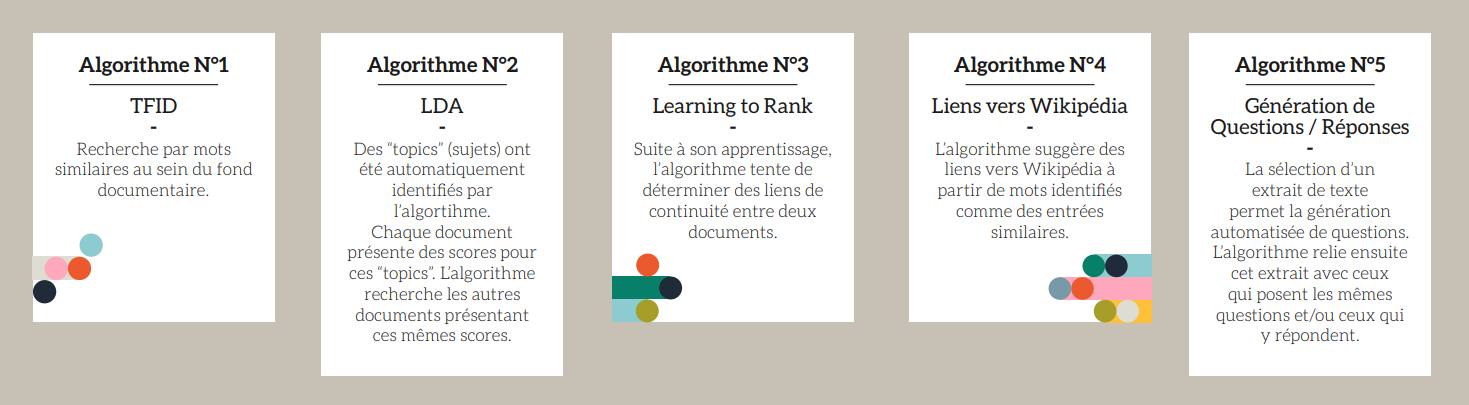
\includegraphics[width=0.8\textwidth]{images/image27.png}
	\caption{Les différents algorithmes à l'oeuvre dans \textit{Archival}}
	\label{fig:image27}
\end{figure}

\begin{center}
	Depuis : Agnola, Azémard, de Silva
\end{center}


L’approche est dite de la \enquote{boite transparente} (\textit{glass box})\footnote{Par opposition à l’effet boite noire (black box) souvent décrit pour évoquer la difficulté de compréhension des processus liés à l’intelligence artificielle\index{Intelligence artificielle}.}, dans laquelle l’enjeu n’est plus uniquement le résultat, mais le processus qui y mène\footcite[p. 47]{besnehard_evaluer_nodate}. L’objectif pour l’équipe du projet est d’expliquer en détail ce que fait chaque algorithme pour que les usagers comprennent les biais et problématiques posées ; de même qu’on a appris que pour trouver le journal \enquote{le voleur} dans un moteur de recherche il fallait, pour éviter les problématiques d’homonymie ajouter \enquote{journal} à notre requête, les chercheurs auront à apprendre les biais et problématiques de l’intelligence artificielle\index{Intelligence artificielle} grâce à une démarche d’explicabilité des projets. Cette notion est donc autant du côté des producteurs et des créateurs d’interfaces qui doivent les rendre les plus transparentes possibles que du côté des utilisateurs qui doivent s’acculturer au numérique et comprendre ses écueils. On a là un exemple d’explicabilité dite globale, c’est-à-dire que ce qui est donné à comprendre à l’usager est le fonctionnement général de l’algorithme, à la différence du niveau local où on expliquerait chacune des décisions que ce dernier prendra\footcite[p. 15]{maxwell_comment_2020}.

\subsection{L'accessibilité numérique}

Dans le rapport sur la découvrabilité en ligne des contenus culturels francophones, déjà cité plusieurs fois, qui est l’illustration des politiques culturelles mises en œuvre pour l’amélioration de cette dernière. Une notion est presque totalement absente : l’accessibilité\index{Accessibilité} numérique. Elle n’est mentionnée qu’une seule fois à la page 25 : \enquote{Par ailleurs, les métadonnées renseignant les fonctionnalités d’accessibilité\index{Accessibilité} disponibles avec le contenu (par exemple, une composante d’audiodescription associée à une vidéo) sont essentielles pour la découvrabilité de ces contenus auprès des personnes en situation de handicap (mental, auditif, visuel, moteur, etc.).} Si ce qui est écrit est tout à fait vrai, il nous semble que c’est une vision un peu restrictive de la question des métadonnées d’accessibilité\index{Accessibilité} et de leur intérêt pour la découvrabilité. Mais avant de poursuivre, prenons le temps de définir ce qu’est l’accessibilité\index{Accessibilité} numérique et ce que cela implique. Selon \enquote{mon parcours handicap}, site d’information pour les personnes en situation de handicap et leurs aidants, l’accessibilité\index{Accessibilité} numérique c’est ce qui permet aux personnes en situation de handicap d’accéder aux contenus d’un site web sans difficulté\footcite{noauthor_accessibilite_nodate}. Cela implique donc quatre notions importantes : la perception par tous les publics (textes alternatifs aux contenus non textuels par exemple) ; l’utilisation (navigation simple et \enquote{logique} pour trouver le contenu même sans le voir) ; la compréhension (création de pages prévisibles, aides à la saisie) et la robustesse (optimisation de la compatibilité)\footcite{noauthor_notion_nodate}. L’accessibilité\index{Accessibilité} ce n’est donc pas simplement le fait de rajouter des textes de remplacements aux images sur un site, c’est un processus qui doit être abordé depuis le design du projet et pendant toute sa durée de vie\footcite{noauthor_accessibilite_nodate} pour prendre en compte tous les publics. Alors qu’entre 4,3 \% et 13,8 \% de la population sont considérés comme handicapés en France (selon le degré de handicap pris en compte, les nombres sont très différents), soit entre 2.8 et 9 millions de personnes\footcite{noauthor_personnes_2022}. Une politique de découvrabilité ne peut donc se passer d’une politique d’accessibilité\index{Accessibilité}.

Loin d’être uniquement, comme on le lit souvent, une contrainte, l’accessibilité\index{Accessibilité} doit être vue comme une opportunité pour les créateurs de sites. Car avoir une démarche de mise en accessibilité\index{Accessibilité} d’un site les oblige à poser la question de sa navigation qui doit être la plus simple et la plus logique possible pour que, notamment, les lecteurs d’écran ne s’y perdent pas. Or, un lecteur d’écran fonctionne exactement de la même manière qu’un \textit{crawler}, ces petits robots qui parcourent automatiquement les sites web pour les indexer afin que les moteurs de recherche puissent les afficher. Plus un site est clair, sa navigation fluide et aisée, mieux le lecteur d’écran pourra le lire et mieux le \textit{crawler} en comprendra la structure, le plan donc meilleure sera l’indexation de votre site et donc son référencement\index{Référencement} et sa repérabilité\index{Repérabilité} sera accrue\footcite{adminat_et_2023}. Par ailleurs, le fait de renseigner les fameux textes de remplacement sur les images permet aussi aux moteurs de recherche de les indexer, et donc de les afficher, améliorant ainsi le référencement\index{Référencement} de ces dernières.

Autre notion importante, rendre un site accessible c’est-à-dire souvent plus clair et plus facile dans sa navigation est aussi utile pour une catégorie de gens souvent oubliés : ceux souffrant de ce qu’on appelle la fracture numérique ou l’illectronisme, qui toucherait plus de 15 \% de la population française en 2021\footnote{Selon des chiffres de l'INSEE \url{https://www.insee.fr/fr/statistiques/7633654}}. Donc, la mise en accessibilité\index{Accessibilité} permet aussi à ces publics qui ont des difficultés à comprendre l’univers numérique de naviguer et d’utiliser plus facilement les sites. Dernier élément à prendre en compte, l’accessibilité\index{Accessibilité} doit aussi se placer du côté des machines et des connexions \textit{internet} : un site web accessible doit donc améliorer son temps de chargement (ce qui améliore aussi son référencement\index{Référencement}), ce qui en plus de le rendre plus facilement consultable pour tous permet d’économiser des ressources matérielles et informatiques et donc de réduire l’impact carbone, grandissant du numérique qui sera l’objet de notre prochaine partie.

\subsection{Et la planète dans tout ça ?}

La fin de la loi de Moore est-elle un motif d’espoir ? C’est en tout cas ce qu’écrit Tristan Nitot, ex-président de Mozilla Europe et personnalité influente du monde du numérique\footcite{nitot_loi_2024}. Mais qu’est-ce que la loi de Moore et pourquoi serait-ce une bonne nouvelle que d’annoncer sa mort ? Formulée il y a bientôt 60 ans (1965) par le co-fondateur d’Intel Gordon Moore qui la résumait par cette phrase : \enquote{le nombre de transistors dans les semiconducteurs [les processeurs] va doubler tous les deux ans à coût constant}\footcite{zotero-301}. Si l’on veut résumer grossièrement, un transistor est une espèce d’interrupteur qui peut être commandé, plus ils sont nombreux plus un processeur peut faire de calculs, puisqu’ils sont responsables de ces derniers : les 0 et 1 du binaire étant en fait l’état des transistors selon qu’ils sont éteints ou allumés\footcite{2024e}. Si la loi de Moore se vérifie toujours si on regarde le nombre de transistors, actuellement de 50 milliards dans nos processeurs, en observant plutôt la puissance de calcul, elle ne se vérifie plus, car si le nombre de transistors est effectivement relié à cette variable, d’autres paramètres entrent en ligne de compte.

Au final, comme l’écrit l’auteur, cela peut devenir un motif d’optimisme. Car le corollaire de la loi de Moore, la loi de Wirth, qui se résume elle aussi en une phrase \enquote{ce qu’Intel vous donne, Microsoft le reprend} qui nous montre que l’augmentation de puissance des processeurs qui s’est observée depuis des années s’est toujours accompagnée d’un ralentissement de nos applications et pages web qui sont, par exemple, 150 fois plus lourdes qu’il y a 25 ans\footcite[§ 8]{nitot_loi_2024}. Par ailleurs, si la loi de Moore stipulait que le coût devait rester constant, ce n’est plus vraiment le cas, les consommations étant en constante augmentation de même que les prix\footcite[§ 4- § 6]{nitot_loi_2024}. On avait donc une fuite en avant avec des processeurs qui devenaient de plus en plus puissants avec des applications de plus en plus gourmandes : ce n’était évidemment pas soutenable scientifiquement parlant (la réduction des tailles de transistors ayant tout de même des limites de même que leur refroidissement qui est le principal problème aujourd’hui), mais aussi écologiquement parlant. On préférait toujours développer des fonctionnalités supplémentaires à des applications, sans jamais prendre le temps de les optimiser, ces dernières étaient donc de plus en plus lourdes et de moins en moins optimisées, ce qui était possible avec la loi de Moore ne le sera plus bientôt\footcite[§ 9]{nitot_loi_2024}. Ce faisant, nos ordinateurs personnels, qui étaient avant constamment ralentis et mis au ban, car trop peu performants, pourraient dans le futur être plus durables avec la fin de la loi de Moore.

Quand on note que 90 \% de l’impact carbone du numérique était causé en 2021 par son cycle de fabrication, qui en plus nécessite des matériaux rares, extraits souvent dans des conditions inhumaines\footcite[§ 16]{guillard_chapitre_2021} : on peut se dire, et à raison, que la conservation de nos terminaux personnels le plus longtemps possible est essentielle. Quant au reste de l’impact carbone du secteur, il est lié à son usage, et 80 \% sont le fait du visionnage de vidéos. Il ne faut donc pas éluder cette question de l’usage, car, par ailleurs, entre 2021 et 2024, la tendance est en train de s’inverser avec un impact carbone de 78 \% du côté de la fabrication et de 22 \% du côté de la phase d’utilisation\footcite{noauthor_quelle_nodate}. Les causes ? L’explosion de l’usage de la vidéo à la demande et du média sur les réseaux sociaux (penser à \textit{Tik Tok} par exemple) d’une part, et de l’autre — et on l’avait simplement évoqué dans notre partie 1 — l’impact grandissant de l’intelligence artificielle\index{Intelligence artificielle} générative. Ces dernières, et leurs milliards de paramètres (1000 milliards dans GPT-4\footnote{Selon les estimation les plus probables (\textit{in} Wikipédia, GPT-4)}) consomment des quantités d’énergie extrêmement importantes, car elles ont besoin d’une puissance de calcul immense pour fonctionner. C’est valable pendant leur phase d’entrainement, par exemple GPT-3 et ses 175 millions de paramètres a généré 552 tonnes d’équivalent CO2\footcite{noauthor_pourquoi_2023}, en sachant que si l’on se fie aux interprétations des Nations unies dans leur rapport \enquote{emission gap report 2020}\footnote{\textit{in} \url{ https://bonpote.com/objectif-2-tonnes-vrai-defi-ou-mauvaise-cible/}}, pour limiter le réchauffement à 1,5°C (et donc respecter l’accord de Paris pour le climat) nous devrions tous émettre environ 2 tonnes par an : cet entrainement (et encore d’un modèle ancien faute de données récentes) est donc loin d’être négligeable. C’est évidemment aussi valable pendant la phase d’utilisation (et sûrement bien plus) des modèles, et ici aussi les chiffres font défaut, on peut noter que Google a augmenté l’année dernière son empreinte carbone de 48 \% et Microsoft (qui héberge \textit{OpenAI}) de 39 \% (alors que les émissions du géant américain étaient en baisse depuis quelques années)\footcite{noauthor__nodate}. Quand on sait que les émissions mondiales du secteur représentaient 3,7 \% en 2021 et devraient représenter 9 \% d’ici à 2052, c’est-à-dire autant que les voitures, il ne faut pas négliger cet aspect, même dans une politique de découvrabilité. Car cette dernière a besoin, elle aussi, de beaucoup de données : pour générer les visualisations de données et interfaces nouvelles et généreuses vues dans la partie 2 par exemple, mais aussi pour stocker et rendre disponible au plus grand nombre le patrimoine numérisé. Il ne faut donc pas que les institutions fassent une \enquote{course en avant} dans le domaine et numérisent l’intégralité de leurs collections dans l’objectif de la faire découvrir en totalité, mais plutôt qu’elles le fassent — comme c’est plutôt le cas actuellement il faut le souligner — de façon raisonnée et sobre. \enquote{Combien faut-il numériser de missels du XIX\textsuperscript{e} siècle pour témoigner de la piété de la société à cette époque ?}\footcite[p. 21]{bermes2024}. Dans le cas du patrimoine audiovisuel par ailleurs, il faut aussi veiller à ne pas forcément proposer la qualité d’image maximale (déjà ça n’a pas toujours de sens au vu des conditions dans lesquelles étaient regardées les émissions de l’époque), mais plutôt l’adapter au support de lecture et à l’usage qui en sera fait.

